\section{Level 1 Pipelines}

\subsection{Single Frame Processing Pipeline (\wbsSFM)}

\subsubsection{Key Requirements}

Single Frame Processing (SFM) Pipeline is responsible for reducing raw image data to \emph{calibrated exposures}, and detection and measurement of \Sources (using the components functionally a part of the Object Characterization Pipeline).
\\

SFM pipeline functions include:
%
\begin{itemize}
    \item Assembly of per-amplifier images to an image of the entire CCD;
    \item Instrumental Signature Removal;
    \item Cosmic ray rejection and snap combining;
    \item Per-CCD determination of zeropoint and aperture corrections;
    \item Per-CCD PSF determination;
    \item Per-CCD WCS determination and astrometric registration of images;
    \item Per-CCD sky background determination;
    \item Source detection.
\end{itemize}

Calibrated exposure produced by the SFM pipeline must possess all information necessary for measurement of source properties by single-epoch Object Characterization algorithms.

It shall be possible to run this pipeline in two modes: a ``fast" mode needed in nightly operations for Level 1 data reductions where no source characterization is done beyond what's required for zero-point, PSF, sky, and WCS determination (image reduction); and a ``full" mode that will be run for Level 2 data reductions.

\subsubsection{Baseline Design}

Single Frame Processing pipeline will be implemented as a flexible framework where different data can be easily treated differently, and new processing steps can be added without modifying the stack code.
\\

It will consist of three primary components:
%
\begin{itemize}
    \item A library of useful methods that wrap a small number of atomic operations (e.g., {\tt interpolateFromMask}, {\tt overscanCorrection}, {\tt biasCorrection}, etc.) % RHL things like overscanCorrection aren't atomic (or at least, they use afw::math and afw::cameraGeom primitives)
    \item A set of classes ({\tt Task}s) that perform higher level jobs
    (e.g., {\tt AssembleCcdTask}, or {\tt FringeTask}), and a top level class to apply corrections to the input data in the proper order. This top level class can be overridden in the instrument specific {\tt obs\_*} packages, making the core SFM pipeline camera agnostic.
    \item A top-level Task to run the SFM pipeline.
\end{itemize}

In the paragraphs to follow, we describe the adopted baseline for key SFM algorithms. If not discussed explicitly, the algorithmic baseline for all other functionallity is assumed to be the same as that used by SDSS \emph{Photo} pipeline \cite{LuptonPhoto}.

\paragraph{Instrumental Signature Removal:}

The adopted pipeline design allows for straightforward addition of correction for instrumental effects that will be discovered in the as-built Camera. The effects currently baselined to be corrected are:

\begin{itemize}
\item Bias: A master bias frame, created from a set of overscan corrected zero length exposures, is subtracted from the image to correct for 2D structure in the bias level. For each exposure, overscan columns will be averaged and fit with a 1D function and subtracted row by row to account for time variable bias level.

\item Assembly: CCDs will be assembled by trimming the prescan and/or overscan rows and columns from amplifier images and storing them into a Image object.

\item Dark current: A master dark frame created from a set of bias corrected exposures taken with the shutter closed is scaled to the science image exposure time and subtracted to correct for 2D structure in the dark current.

\item Cross-talk: Cross talk is generated by interaction of fields produced by the current in physically proximate electronic components. This results in bright features from one amp showing up in other. Correction is to subtract each aggressor amp (possibly flipped) modulated by a measured coefficient from the victim amp. The implementation may assume the cross-talk is small enough to be correctable by first order correction only.

\item Non-linearity: CCDs do not have perfectly linear response. At both almost empty and almost full well the response can become non-linear. Given a measurement of the linearity of the CCD response, along with any temperature dependence, the data values will be corrected to linear response by simple mapping and interpolation.

\item Flat-field: The correction is a division by the normalized master flat. The master flat will be generated assuming a nominal flat spectrum for all sources. Photometric corrections will be applied downstream on a source by source basis given an SED for each source.

\item Fringing: Fringe parerns are an interference effect that result from the sharp emission lines in the night sky spectrum. This effect is the strongest in redder bands. The best fit modeled fringe pattern, constructed from monochromatic flats assuming a low-dimensional parametrization of the night sky emission spectrum, will be subtracted from the image.

\item Cosmic ray rejection and snap combining: Exposures will be taken in pairs separated by the readout time. The two images and the expected statistics on those images are used to reject pixels that are significant outliers. Once cosmic rays are flagged the two snaps will be added to produce an image with a longer effective exposure.  % RHL There'll probably also be a significant morphological component.  Esp. if we want snap-to-snap transients...
\end{itemize}

\paragraph{PSF determination:} We will run separate algorithms to select candidate stars and determine the point-spread function (PSF, the light distribution for a point source, a critical ingredient to understanding the data and measuring accurate fluxes and shapes).  Both the star selector and PSF determiner algorithms will be pluggable Python modules, so that different algorithms can be run as desired for different analysis needs.

Three selectors will be implemented. % RHL I bet that these will change dramatically before construction.  I was tempted to change ``will be implemented'' to ``will be implemented initially'' but didn't.
The ``second-moment'' star selector will build a histogram of the X and Y second moments of flux, search for a peak, and select sources in the peak as point source candidates.  The ``catalog'' star selector, in contrast, will make use of an external catalog of point sources and use astrometric matching to select point source candidates.  The ``objectSize'' star selector will identify point source candidates from the cluster of sources with similar sizes regardless of magnitude.  When selecting point source candidates by size (i.e., for the ``second-moment'' and ``objectSize'' algorithms), the sizes will be corrected by the known optical distortion of the camera.  % RHL objectSize has superceded secondMoment already.
\\

Given the irregularly sampled grid of PSFs represented by selected stars, the variation of the PSF across the CCD will be determined. The baselined ``principal-components'' PSF (pcaPsf) determiner performs a singular value decomposition (also known as a principal components analysis, or PCA) on the point-source candidates in pixel space to produce a set of eigen-images.  Using the dominant eigen-images, it constructs polynomial interpolants for their relative weights.  This produces a spatially-varying PSF model that captures the most important changes in the PSF over the CCD.
\\

These algorithms are intended to be sufficient to enable Level 1 processing. More advanced PSF determination algorithms will be developed in the PSF Estimation Pipeline (\wbsPSF).
% RHL We'll have to be careful, as I think these fluxes/positions are the inputs into global calibration

\paragraph{Sky Background Determination:}

We will estimate the smooth sky background by measuring the background level in cells (typically 256 or 512 pixels square) % RHL I'm sure 256 will be too small.  512 may well be too.
using (by default) a clipped mean, and ignoring pixels that are part of detected sources.  An interpolating spline (an Akima spline, by default) will be constructed to estimate the background level in each pixel. Backgrounds will be possible to estimate simultaneously over multiple sensors, including the full focal plane.

Background models will be saved, for later subtraction or restoration (e.g., in background matching, as implemented by the Coaddition Pipeline, \wbsCoadd).

\paragraph{WCS determination and image registration}

The absolute World Coordinate System (WCS) will be determined using an \emph{astrometry.net} type algorithm \cite{Lang09}, seeded with the approximate position of the boresight.  % RHL I doubt if we'll use a.n in production (except as a fallback when all else fails)

This module will also include the capability to perform relative registration of a set of images to enable coaddition and image differencing, using the \emph{meas\_mosaic} registration algorithm developed by Furusawa et al. \cite{Furusawa14} as the baseline.

\subsubsection{Constituent Use Cases and Diagrams}

Assemble CCD; Determine Aperture Correction; Determine PSF; Remove Instrument Signature; Detect Sources; Determine Photometric Zeropoint; Measure Single Visit Sources; Determine WCS; Sum Exposures, Combine Raw Exposures, Remove Exposure Artifacts; Determine Sky Background Model; Calibrate Exposure; Process Raw Exposures to Calibrated Exposure; Perform Single Visit Processing;

\subsubsection{Prototype Implementation}

A prototype implementation of all major components of SFM baseline design has been completed in LSST Final Design Phase. The achieved accuracy is comparable to state-of-the art codes today (e.g., SDSS, SExtractor). We expect it will be possible to transfer a significant fraction of the existing code into Construction, with continued improvement to meet LSST accuracy requirements.
\\

WCS determination and image registration modules are an exception, and will require extensive redesign and rewrite. The sky determination module will have to be enhanced to support multi-CCD fitting capability.
\\

The prototype codes are available in the following repositories: \url{https://github.com/lsst/ip_isr}, \url{https://github.com/lsst/meas_algorithms}, \url{https://github.com/lsst/meas_astrom}, \url{https://github.com/lsst-dm/legacy-meas_mosaic}, \url{https://github.com/lsst/pipe_tasks}.

\clearpage

\subsection{Image Differencing Pipeline (\wbsDiffim)}

\subsubsection{Key Requirements}

The image differencing pipeline shall difference a visit image against a deeper template, and detect and characterize sources in the difference image in the time required to achieve the 60 second design goal for Level 1 alert processing (current timing allocation: 24 seconds). The algorithms employed by the pipeline shall result in purity and completeness of the sample as required by the \DMSR\@. Image differencing shall perform as well in crowded as in uncrowded fields.

\subsubsection{Baseline Design}
\label{sec:diffimDesign}

\begin{figure}
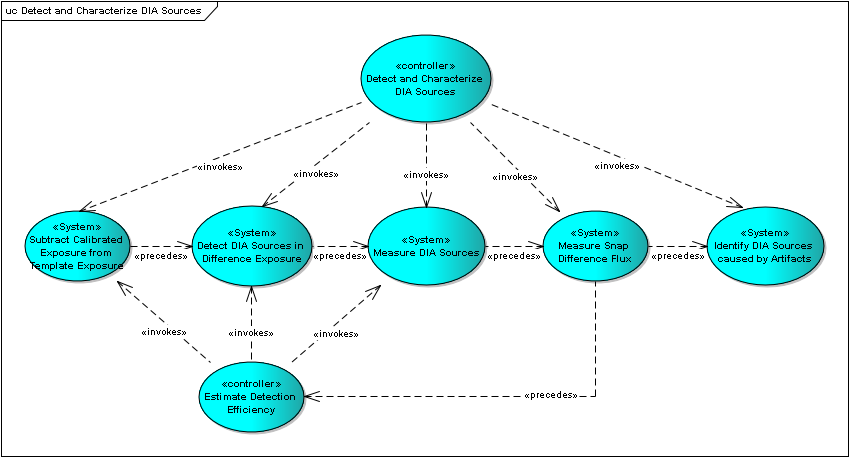
\includegraphics[angle=0,scale=0.44]{figures/detect_and_characterize_dia_sources.png}
\caption{Image Differencing Pipeline Use Case Diagram\label{fig:diffimUML}}
\end{figure}

The Image Differencing pipeline will difference, detect, and deblend objects in the resulting image using the ``preconvolution'' algorithm as described in Becker et al. \cite{Becker13}.
Differencing will be performed against a deeper template, and differential chromatic refraction (DCR) will be handled by having templates in several bins of airmass.

All \DIASource measurements described in the \DPDD, including post-processing such as variability characterization, will be performed for all sources detected in this manner. The measurements will be performed on the pre-convolved likelihood image. This involves invoking some algorithms defined in the Object Characterization Pipeline (\wbsObjChar{}) as well as algorithms specific to difference images, which are defined in this WBS (see \S\ref{alg:dipole}).
\\

If necessary a \emph{spuriousness metric} using machine-learning techniques (e.g., Bloom et al. \cite{Bloom12}) will be developed to help in the discrimination of real sources from those caused by artifacts.
\\

Details of this baseline design have been captured in the \uc{Detect and Characterize DIA Sources} and related diagrams, presented in Figure~\ref{fig:diffimUML}.

\paragraph{Dipole model fit}
\label{alg:dipole}

The pipeline shall be capable of fitting a dipole object model, as described in the \DPDD{}. The baseline algorithm is analogous to that employed by the bulge-disk model fit (\S\ref{alg:bulgedisk}), but with the model being a mixture of positive and negative point sources, instead of S\'ersic profiles.

\subsubsection{Constituent Use Cases and Diagrams}

Subtract Calibrated Exposure from Template Exposure; Identify DIA Sources caused by Artifacts; Perform Precovery Forced Photometry; Measure DIA Sources; Detect DIA Sources in Difference Exposure; Measure Snap Difference Flux; Perform Difference Image Forced Photometry; Calculate DIA Object Flux Variability Metrics; Fit DIA Object Position and Motion;

\subsubsection{Prototype Implementation}

A prototype implementation partially implementing the baseline design has been completed in the LSST Final Design Phase. It includes detection, centroiding, aperture and PSF photometry, and adaptive shape measurement.
% RHL I don't think it does, or at least not correctly.  I think that they just ran the standard algorithms as black boxes rather than adjusting them allow for the preconvolution.
This implementation was used to benchmark the speed of the image differencing code and examine the expected levels of false positives. Deblending on difference images, fits to trailed sources, and dipole fits were not prototyped. The final report on prototype design and performance can be found in Becker et al. (\url{http://ls.st/x9f}).
\\

The prototype code is available at \url{https://github.com/lsst/ip_diffim}. The current prototype, while functional, will require a partial redesign to be transfered to construction to address performance and extensibility concerns.

\clearpage

\subsection{Association Pipeline (\wbsAssocP)}

\subsubsection{Key Requirements}

The Association Pipeline has two key responsibilities: i) it must be able to associate newly discovered \DIASources with previously known \DIAObjects and \SSObjects, and ii) it must be able to associate \DIAObjects with known \Objects from the Level 2 catalogs.

\subsubsection{Baseline Design}

The baseline design for \DIASources to \DIAObject association and \DIAObject to \Object association is to use simple nearest-neighbor search while taking proper motions and positional errors ellipses into account.

For matches to \SSObjects, the \SSObject's ephemeris are to be computed by NightMOPS (functionally a part of the Moving Object Pipeline, \wbsMOPS). Matching to the computed ephemeris is to be performed as if they were \DIAObjects.

When Level 1 data is reprocessed, a more sophisticated clustering algorithm \cite{Ankerst99} will be employed.

\subsubsection{Constituent Use Cases and Diagrams}

Create Instance Catalog for Visit; Associate with Instance Catalog;
Perform DIA Object Association; Perform DIA Source Association;

\subsubsection{Prototype Implementation}

Prototype implementation of the baseline design has been completed in LSST Final Design Phase. The nearest-neighbor matching has been implemented as a part of the Application Framework, while clustering using OPTICS resides in the database-related ingest modules.
\\

The prototype code is available at \url{https://github.com/lsst-dm/legacy-ap}. The current prototype, while functional, will require a partial redesign in Construction to address scalability and performance.

\clearpage

\subsection{Alert Generation Pipeline (\wbsAP)}

\subsubsection{Key Requirements}

Alert Generation Pipeline shall take the newly discovered \DIASources and all associated metadata as described in the \DPDD, and generate alert packets in \VOEvent format. It will transmit these packets to VO Event Brokers, using standard IVOA protocols (eg., VOEvent Transport Protocol; VTP\@. End-users will primarily use these brokers to classify and filter events for subsets fitting their science goals.
% RHL I thought that we were being careful to say we'll use whatever's the standard, e.g. VO?

To directly serve the end-users, the Alert Generation Pipeline shall provide a basic, limited capacity, alert filtering service. This service will run at the LSST U.S. Archive Center (at NCSA). It will let astronomers create simple filters that limit what alerts are ultimately forwarded to them. These \emph{user defined filters} will be possible to specify using an SQL-like declarative language, or short snippets of (likely Python) code.

\subsubsection{Baseline Design}

The baseline design is to adopt and upgrade for performance and functionallity the Skyalert package (\url{http://lib.skyalert.org/skyalert/}).

\subsubsection{Constituent Use Cases and Diagrams}

Distribute to Subscribed Brokers; Distribute to Subscribed Users; Generate Alerts;
Generate and Distribute Alerts;

\subsubsection{Prototype Implementation}

No prototype implementation has been developed by LSST, as the Skyalert package (\url{http://lib.skyalert.org/skyalert/}) was found to be mature enough to baseline the architecture and estimate costs.

\clearpage

\subsection{Moving Object Pipeline (\wbsMOPS)}

\subsubsection{Key Requirements}

The Moving Object Pipeline System (MOPS) has two responsibilities within LSST Data Management:

\begin{itemize}
    \item First, it is responsible for generating and managing the Solar System\footnote{Also sometimes referred to as `Moving Object'} data products. These are Solar System objects with associated Keplerian orbits, errors, and detected \DIASources. Quantitatively, it shall be capable of detecting 95\% of all Solar System objects that meet the findability criteria as defined in the \OSS\@. The software components implementing this function are known as {\bf \em DayMOPS}.
    \item The second responsibility of the MOPS is to predict future locations of moving objects in incoming images so that their sources may be associated with known objects; this will reduce the number of spurious transient detections and appropriately flag alerts to detections of known Solar System objects.  The software components implementing this function are known as {\bf \em NightMOPS}.
\end{itemize}

\subsubsection{Baseline Design}

The baseline NightMOPS design is to adopt and adapt an existing ephemeris computation pipeline such as OrbFit\footnote{\url{http://adams.dm.unipi.it/orbfit/}} or OpenOrb\footnote{\url{https://github.com/oorb/oorb}}. The baseline DayMOPS design uses Kubica et al. \cite{Kubica05} algorithms to identify and link Solar System object candidates.
\\

The design of these components are explained in detail in the MOPS Design Document (\MOPSD).

\subsubsection{Constituent Use Cases and Diagrams}

Process Moving Objects;
Fit Orbit; Prune Moving Object Catalog; Perform Precovery; Recalculate Solar System Object Properties; Link Tracklets into Tracks; Find Tracklets;

\subsubsection{Prototype Implementation}

A prototype implementation implementing the key components of DayMOPS baseline design has been completed in LSST Final Design Phase. NightMOPS has not been extensively prototyped, as it is understood not to be an area of significant uncertainty and risk. An extensive report on MOPS prototyping and performance is available as a part of the MOPS Design Document (\MOPSD).
\\

Prototype MOPS codes are available at \url{https://github.com/lsst/mops_daymops} and \url{https://github.com/lsst/mops_nightmops}. We expect it will be possible to transfer a significant fraction of the existing code into Construction. Current DayMOPS prototype already performs within the computational envelope envisioned for LSST Operations, though it does not yet reach the required completeness requirement.
